%%%%%%%%%%%%%%%%%%%%%%%%%%%%%%%%%%%%%%%%%%%%%%%%%%%%%%%%%%%%%%%%%%%%%%%%%%%%%%%%
%2345678901234567890123456789012345678901234567890123456789012345678901234567890
%        1         2         3         4         5         6         7         8

%\documentclass[letterpaper, 10 pt, conference]{ieeeconf}  % Comment this line out
                                                          % if you need a4paper
\documentclass[a4paper, 10pt, conference]{ieeeconf}      % Use this line for a4
                                                          % paper

\IEEEoverridecommandlockouts                              % This command is only
                                                          % needed if you want to
                                                          % use the \thanks command
\overrideIEEEmargins
% See the \addtolength command later in the file to balance the column lengths
% on the last page of the document



% The following packages can be found on http:\\www.ctan.org
%\usepackage{graphics} % for pdf, bitmapped graphics files
%\usepackage{epsfig} % for postscript graphics files
%\usepackage{mathptmx} % assumes new font selection scheme installed
%\usepackage{times} % assumes new font selection scheme installed
%\usepackage{amsmath} % assumes amsmath package installed
%\usepackage{amssymb}  % assumes amsmath package installed

\title{\LARGE \bf
Decentralized Communications for Self-regulated\\ Division of Labour in Robot Society
}

\author{ Md Omar Faruque Sarker and Torbjorn Dahl\\
         %\thanks{This research has been funded by the Engineering and Physical Sciences 				Research Council (EPSRC), UK, grant reference EP/E061915/1.}%
        Robotic Intelligence Lab, Newport Business School\\
		University of Wales, Newport, Allt-yr-yn Campus\\ 
		Allt-yr-yn Avenue, Newport, NP205XR, UK\\
		{\tt\small Mdomarfaruque.Sarker@newport.ac.uk}\\ 
		{\tt\small Torbjorn.Dahl@newport.ac.uk}      
}

%\author{Huibert Kwakernaak and Pradeep Misra% <-this % stops a space
%\thanks{This research has been funded by the Engineering and Physical Sciences Research Council (EPSRC), UK, grant reference EP/E061915/1.}% <-this % stops a space
%%\thanks{H. Kwakernaak is with Faculty of Electrical Engineering, Mathematics and Computer Science,
%%        University of Twente, 7500 AE Enschede, The Netherlands
%%        {\tt\small h.kwakernaak@autsubmit.com}}%
%%\thanks{P. Misra is with the Department of Electrical Engineering, Wright State University,
%%        Dayton, OH 45435, USA
%%        {\tt\small pmisra@cs.wright.edu}}%
%}


\begin{document}


\maketitle
\thispagestyle{empty}
\pagestyle{empty}


%%%%%%%%%%%%%%%%%%%%%%%%%%%%%%%%%%%%%%%%%%%%%%%%%%%%%%%%%%%%%%%%%%%%%%%%%%%%%%%%
\begin{abstract}

Distributed local communication is one of the essential means by which various social insects achieve their self-regulatory division of labour. Unlike centralized static communication, this communication mode enables individuals to respond to local changes more quickly and it generally produces steady-state convergence of self-regulated division of labour (DoL) in social insects. However, realizing this kind of communication in a distributed multi-robot system (DMRS) is not as straight forward as a centralized one. From a robot controller's point of view, it is not easy to determine how often or how much dynamic peer-to-peer (P2P) communication  is needed to maintain system's convergence of division of labour. In this paper, we address these questions: first by describing our model of local communication based DMRS with two different communication radii that shows a steady-state convergence of self-regulated DoL. Then we compare this system with our centralized communication based DMRS. All experiments on these systems  have been done with 16 physical E-puck robots in an area of about 4$m^2$. Results from these experiments suggest that faster and more stable convergence can be obtained by setting a smaller P2P communication radius where a robot locally exchanges signals with a minimum number of its closest peers.

\end{abstract}


%%%%%%%%%%%%%%%%%%%%%%%%%%%%%%%%%%%%%%%%%%%%%%%%%%%%%%%%%%%%%%%%%%%%%%%%%%%%%%%%
\section{INTRODUCTION}
\label{sec:intro}
%\vspace{2mm}
Multi-agent task allocation or division of labour (DoL) is a challenging research issue in the field of multi-agent and multi-robot systems e.g., swarm robotics \cite{RefSwarm}. In order to address this issue, existing approaches e.g., predefined (off-line) and emergent (real-time) task-allocation, fail to scale well with large number of agents. Typically, increased communication interference and decreased bandwidth among agents are major causes of this problem. Unlike the swarm robotic approach, which is inspired by biological systems alone and commonly aims for minimal intelligence agents, we propose to solve DoL in multi-agents based on a set of observed generic rules of DoL from biological and human social systems. These bottom-up rules describe the phenomena of self-regulated DoL in terms of attractive fields between agents and tasks. The concrete form of these rules, termed as \textit{attractive filed model} (AFM) \cite{RefElsa}, offers a scalable solution to the above DoL problem. Unlike having strong dependence to communication mediums by most of the existing approaches, our model states that self-regulatory DoL can be established by AFM without maintaining a strong form of on-line communication. 
%\vspace{4mm}
We have investigated the performance of two different communication strategies for self-regulated DoL among a larger robot teams: centralized and local. These forms of communications typically resemble to message broadcast and peer-to-peer (P2P) communications respectively.


%%%%%%%%%%%%%%%%%%%%%%%%%%%%%%%%%%%%%%%%%%%%%%%%%%%%%%%%%%%%%%%%%%%%%%%%%%%%%%%%
\section{Modeling}
\label{sec:model}
\subsection{Model for Self-Regulatory DoL}
Our model of self-regulated DoL is based on AFM. It provides us a generic framework for implementing self-regulatory DoL in robots. Here we briefly describe how this model gives our robots self-regulatory DoL behaviours, particularly task-specialization, concurrency, flexibility and robustness.
Let us consider a manufacturing shop floor scenario where N number of mobile robots are required to attend to M number of shop tasks spread over a fixed area A. Let these tasks be represented by a set of small rectangular boxes resembling to manufacturing machines. Let $R_1$, $R_2$ … $R_n$ be the set of all robots and $J_1$, $J_2$ … $J_m$ be the set of all tasks. Each task $j$ has an associated task-urgency $\phi_j$ that indicates its relative importance over time. If a robot attends to a task $j$ in x$^{th}$ time-step, value of $\phi_j$ will decreases by a small amount $\delta_\phi$ in (x+1)$^{th}$ time-step. On the other hand, if a task has not been served by any robot in x$^{th}$ time-step,  $\phi_j$  will increase by another small amount in (x+1)$^{th}$ time-step. In order to complete a shop task $J_1$, a robot $R_1$ needs to reach within a fixed boundary $D_j1$ of $J_1$. If a robot completes a task $j$ we say that it learns about it and this will increase robot's likelihood of selecting that task in next step. We call this variable affinity of a robot to that task as its sensitization $k_j$ . If a robot does not do a task $j$ for some time, we say that it forgets about $j$ and $k_j$ has been decreased.\\
According AFM, all robots will establish attractive fields to all tasks due to the presence of a system-wide continuous flow of information. The strength of these attractive fields called stimulus will vary according to the distances between robots and tasks, task-urgencies and corresponding  sensitizations of robots. This is encoded in Eq. \ref{eqn1}.
%\addtolength{\abovedisplayskip}{-15mm} 
\begin{small}
\begin{multicols}{2} 
\begin{equation}
S_{j}^{i} = tanh\{\frac{k_{j}^{i}}{d+\delta } \phi _{j}\}
\label{eqn1}
\end{equation}
\vspace*{0.25cm}
\begin{equation}
P_{j}^{i} = \frac{S_{j}^{i}}{\sum_{j}^{}S_{j}^{i}}
\label{eqn2}
\end{equation}
\end{multicols}
\end{small}
%\addtolength{\belowdisplayskip}{-1mm} 
%\vspace{2mm}
Eqn \ref{eqn1} says that the stimuli of a robot $i$ to a particular task $j$, $(S_{j}^{i})$ depends on robot's spatial distance $d$ to $j$, level of sensitization to that task ($k_{j}^{i}$) and perceived urgency of that task ($\phi _{j}$). We use a vary small value $\delta$ in \ref{eqn1} to prevent  division by zero. The probability of selecting each task has been determined by a probabilistic method outlined in Eq. \ref{eqn2} . 
AFM suggests concurrency of a self-regulatory system by specifying at least two task options: 1) doing a task and 2) doing no task. In robots, the latter can be   be treated as random walking. So in any time-step a robot will choose from M+1 tasks. Let $T_a$ be the allocated time to accomplish a task. If $R_1$ can enter inside the task boundary within $T_a$ time it waits there until $T_a$ elapsed. Otherwise it will select a different task. 

\subsection{Model for Communication}
In order to establish a system-wide continuous flow of information, one needs to implement a  suitable communication system. Here we have presented two models of communication for our above manufacturing shop-floor scenario.
%
%\addtolength{\floatsep}{-25mm}
\begin{figure}[ht]
\begin{minipage}[b]{0.55\linewidth}
\centering
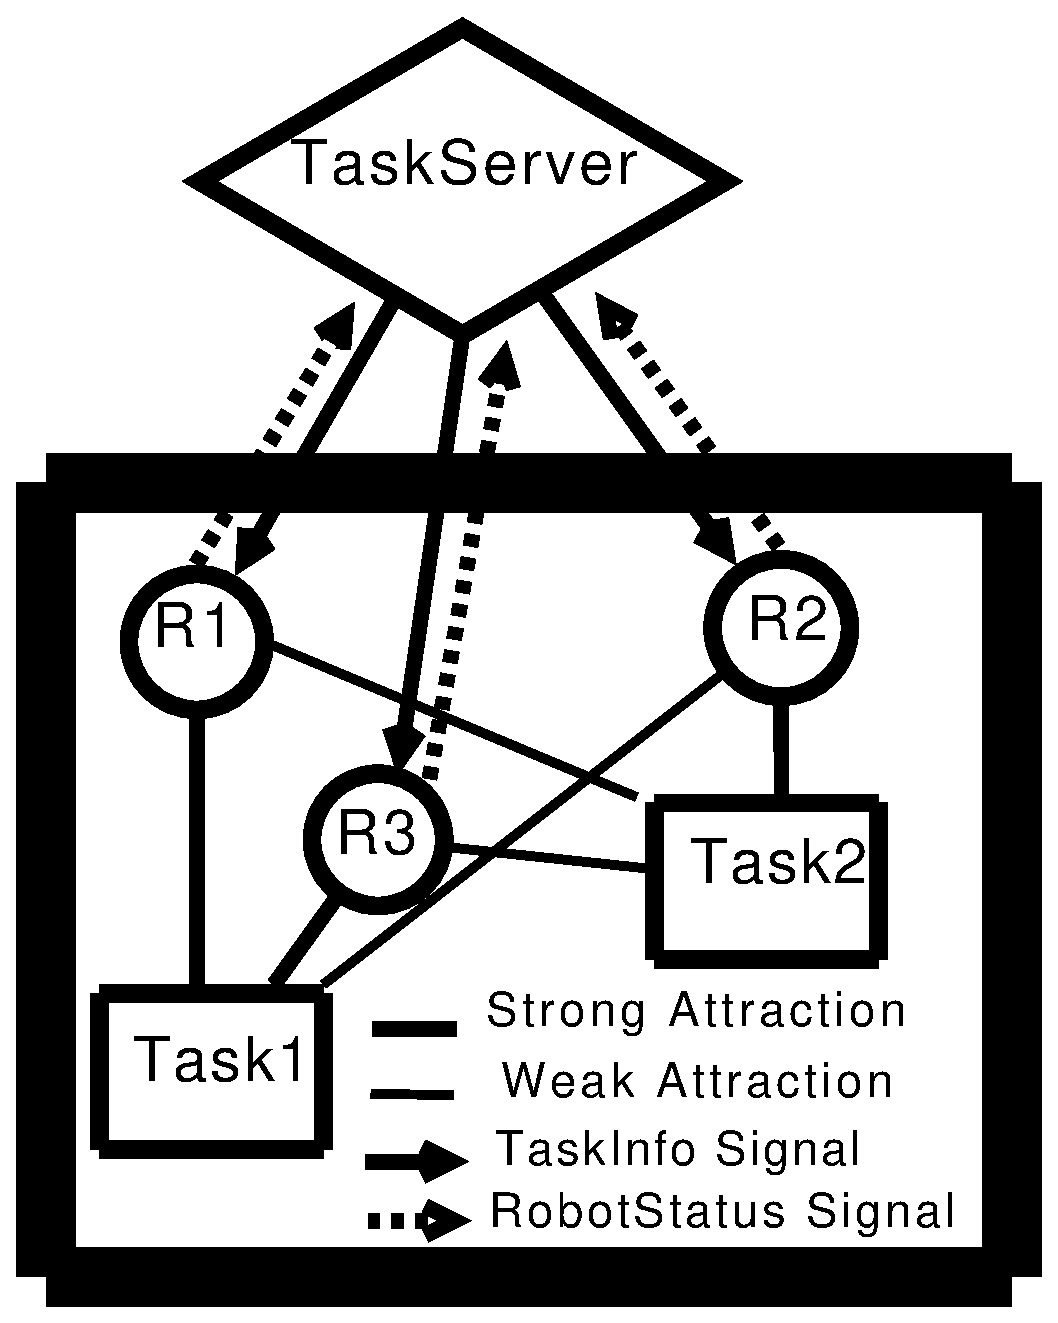
\includegraphics[height=6cm, angle=0]{../dia-files/CentralizedComm.eps}
% figure caption is below the figure
\caption{Centralized communication model}
\label{fig:ccm} % Give a unique label
\end{minipage}
%\hspace{0.5cm}
\begin{minipage}[b]{0.45\linewidth}
\centering
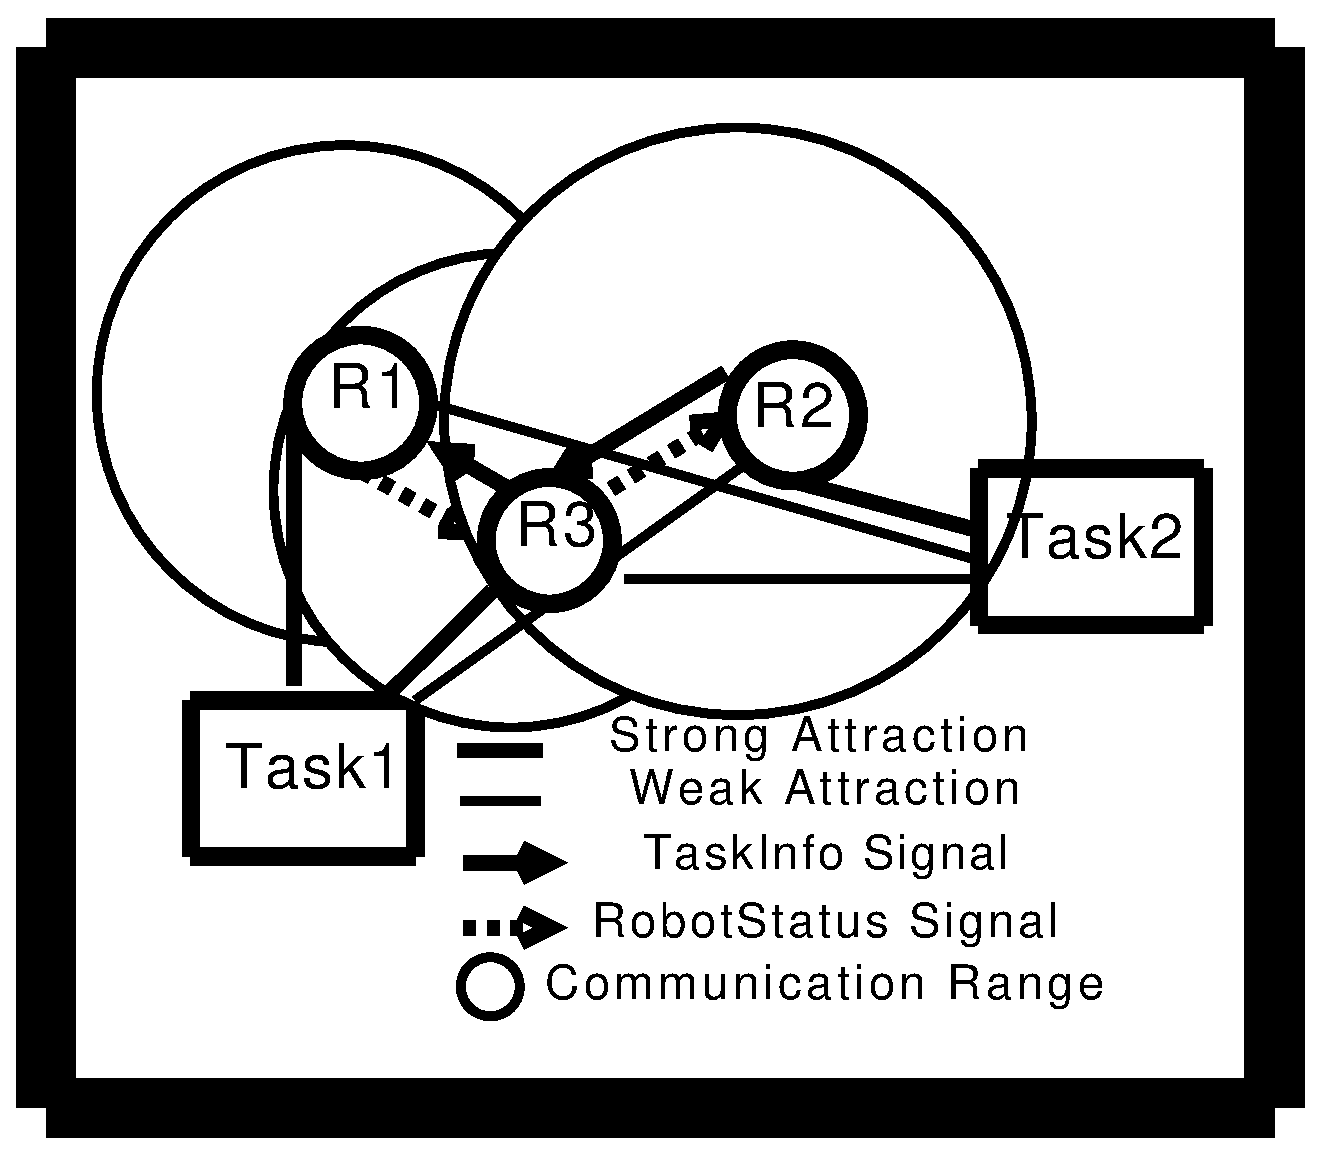
\includegraphics[height=4cm, angle=0]{../dia-files/LocalComm.eps}
% figure caption is below the figure
%\vspace*{0.20cm}
\caption{Local communication model}
\label{fig:lcm} % Give a unique label
\end{minipage}
\end{figure}
%\addtolength{\belowcaptionskip}{-15mm}
%\end{spacing}
%
\paragraph{Centralized Communication Model:}

As shown in Fig. \ref{fig:ccm}, in this model there exists a centralized Task-Server that is responsible for disseminating task information to robots. The content of  task information can be   location of task in the environment, urgency and so on. Task server delivers this information by emitting TaskInfo signals periodically. The method of signal emission depends on a particular communication technology. For example, in a wireless network it can be a message broadcast.
Task-Server has another interface for catching feedback signals from robots. This RobotStatus signal may contain what task a robot is currently doing, its device status and so on.  Task-Server  uses this information to update task information such as, task-urgency. This up-to-date information is sent in TaskInfo signal.
In Fig. \ref{fig:ccm} an initial configuration of this model has been presented. Upon receiving an initial TaskInfo signal robot $R_1$ and $R_2$ shows  strong attractions towards $Task1$ and robot $R_3$ shows strong attraction toward $Task2$. This can be inferred from Eq. \ref{eqn1}. If the initial task urgencies and sensitizations are same for all tasks, a robot will be strongly attracted towards a task that is relatively closer to it.

\paragraph{Local Communication Model:}

This model is based on the P2P communications among robots. Here there is no centralized server to disseminate information but each robot can communicate to its nearby peers within its communication radius, $r_comm$. Here by $r_comm$, we assume that within this distance robots can exchange communication signals reliably without any significant loss of information or delay. A robot $R_1$ is a nearby peer  of robot $R_2$, if spatial distance between $R_1$ and $R_2$ is less than its $r_comm$. 
As shown in Fig. \ref{fig:lcm}, local communication can also give robots similar task information as in centralized communication mode. It shows that  it is not necessary for each robot to communicate with every other robot to get information on all tasks. Since robots can random walk  and explore the environment we assume that for a reasonably high robot to space density, all task will be known to all robots after an initial exploration period. 
In order to update the urgency of a task, robots can estimate the number of robots working on a task either by using their sensory perception (e.g., camera)  or by doing local P2P communication. In Fig. ref{fig:lcm} we have shown that robots exchange both TaskInfo and RobotStatus signals to peers.



%%%%%%%%%%%%%%%%%%%%%%%%%%%%%%%%%%%%%%%%%%%%%%%%%%%%%%%%%%%%%%%%%%%%%%%%%%%%%%%%
\section{ADDITIONAL REQUIREMENTS}

\subsection{Figures and Tables}

Position figures and tables at the tops and bottoms of columns.
Avoid placing them in the middle of columns. Large figures and tables
may span across both columns. Figure captions should be below the figures;
 table captions should be above the tables. Avoid placing figures and tables
  before their first mention in the text. Use the abbreviation ``Fig. 1'',
  even at the beginning of a sentence.
Figure axis labels are often a source of confusion.
Try to use words rather then symbols. As an example write the quantity ``Inductance",
 or ``Inductance L'', not just.
 Put units in parentheses. Do not label axes only with units.
 In the example, write ``Inductance (mH)'', or ``Inductance L (mH)'', not just ``mH''.
 Do not label axes with the ratio of quantities and units.
 For example, write ``Temperature (K)'', not ``Temperature/K''.

\subsection{Numbering}

Number reference citations consecutively in square brackets \cite{c1}.
 The sentence punctuation follows the brackets \cite{c2}.
 Refer simply to the reference number, as in \cite{c3}.
 Do not use ``ref. \cite{c3}'' or ``reference \cite{c3}''.
Number footnotes separately in superscripts\footnote{This is a footnote}
Place the actual footnote at the bottom of the column in which it is cited.
Do not put footnotes in the reference list.
Use letters for table footnotes (see Table I).

\subsection{Abbreviations and Acronyms}

Define abbreviations and acronyms the first time they are used in the text,
even after they have been defined in the abstract. Abbreviations such as
IEEE, SI, CGS, ac, dc, and rms do not have to be defined. Do not use
abbreviations in the title unless they are unavoidable.

\subsection{Equations}

Number equations consecutively with equation numbers in parentheses flush
 with the right margin, as in (1). To make your equations more compact
 you may use the solidus (/), the exp. function, or appropriate exponents.
  Italicize Roman symbols for quantities and variables, but not Greek symbols.
   Use a long dash rather then hyphen for a minus sign. Use parentheses to avoid
    ambiguities in the denominator.
Punctuate equations with commas or periods when they are part of a sentence:
$$\Gamma_2 a^2 + \Gamma_3 a^3 + \Gamma_4 a^4 + ... = \lambda \Lambda(x),$$
where $\lambda$ is an auxiliary parameter.

Be sure that the symbols in your equation have been defined before the
equation appears or immediately following.
Use ``(1),'' not ``Eq. (1)'' or ``Equation (1),''
except at the beginning of a sentence: ``Equation (1) is ...''.

   \begin{figure}[thpb]
      \centering
      %\includegraphics[scale=1.0]{figurefile}
      \caption{Inductance of oscillation winding on amorphous
       magnetic core versus DC bias magnetic field}
      \label{figurelabel}
   \end{figure}

%%%%%%%%%%%%%%%%%%%%%%%%%%%%%%%%%%%%%%%%%%%%%%%%%%%%%%%%%%%%%%%%%%%%%%%%%%%%%%%%
\section{CONCLUSIONS AND FUTURE WORKS}

\subsection{Conclusions}

This is a repeat.
Position figures and tables at the tops and bottoms of columns.
Avoid placing them in the middle of columns. Large figures and tables
may span across both columns. Figure captions should be below the figures;
 table captions should be above the tables. Avoid placing figures and tables
  before their first mention in the text. Use the abbreviation ``Fig. 1'',
  even at the beginning of a sentence.
Figure axis labels are often a source of confusion.
Try to use words rather then symbols. As an example write the quantity ``Inductance",
 or ``Inductance L'', not just.
 Put units in parentheses. Do not label axes only with units.
 In the example, write ``Inductance (mH)'', or ``Inductance L (mH)'', not just ``mH''.
 Do not label axes with the ratio of quantities and units.
 For example, write ``Temperature (K)'', not ``Temperature/K''.


\subsection{Future Works}

This is a repeat.
Position figures and tables at the tops and bottoms of columns.
Avoid placing them in the middle of columns. Large figures and tables
may span across both columns. Figure captions should be below the figures;
 table captions should be above the tables. Avoid placing figures and tables
  before their first mention in the text. Use the abbreviation ``Fig. 1'',
  even at the beginning of a sentence.
Figure axis labels are often a source of confusion.
Try to use words rather then symbols. As an example write the quantity ``Inductance",
 or ``Inductance L'', not just.
 Put units in parentheses. Do not label axes only with units.
 In the example, write ``Inductance (mH)'', or ``Inductance L (mH)'', not just ``mH''.
 Do not label axes with the ratio of quantities and units.
 For example, write ``Temperature (K)'', not ``Temperature/K''.

%%%%%%%%%%%%%%%%%%%%%%%%%%%%%%%%%%%%%%%%%%%%%%%%%%%%%%%%%%%%%%%%%%%%%%%%%%%%%%%%
\section{ACKNOWLEDGMENTS}

The authors gratefully acknowledge the contribution of National Research Organization and reviewers' comments.


%%%%%%%%%%%%%%%%%%%%%%%%%%%%%%%%%%%%%%%%%%%%%%%%%%%%%%%%%%%%%%%%%%%%%%%%%%%%%%%%

References are important to the reader; therefore, each citation must be complete and correct. If at all possible, references should be commonly available publications.

\begin{thebibliography}{99}

\bibitem{c1}
J.G.F. Francis, The QR Transformation I, {\it Comput. J.}, vol. 4, 1961, pp 265-271.

\bibitem{c2}
H. Kwakernaak and R. Sivan, {\it Modern Signals and Systems}, Prentice Hall, Englewood Cliffs, NJ; 1991.

\bibitem{c3}
D. Boley and R. Maier, "A Parallel QR Algorithm for the Non-Symmetric Eigenvalue Algorithm", {\it in Third SIAM Conference on Applied Linear Algebra}, Madison, WI, 1988, pp. A20.

\end{thebibliography}

\end{document}
